% Motivation model diagram Heckhausen and Rheinberg
% Author: Stefan Kottwitz
\documentclass[tikz,border=10pt]{standalone}
\usepackage[normalem]{ulem}
\tikzset{
  centered/.style = { align=center, anchor=center },
     empty/.style = { font=\sffamily\Large, centered, text width=2cm },
       box/.style = { font=\sffamily, fill=green, centered },
    result/.style = { font=\sffamily\scriptsize, fill=black!20, centered},
     arrow/.style = { very thick, color=red, ->, >=Triangle},
}
\newcommand*{\nothing}{Do nothing}

\begin{document}
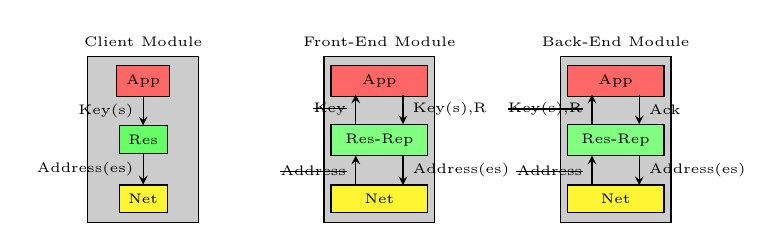
\begin{tikzpicture}
	[layer/.style={rectangle,draw}];
	
	\node (client) at (-3,0) [layer,label={\tiny Client Module},minimum height=60pt,minimum width=40pt,fill=black!20] {};
	\node (front) at (0,0) [layer,label={\tiny Front-End Module},minimum height=60pt,minimum width=40pt,fill=black!20] {};
	\node (back) at (3,0) [layer,label={\tiny Back-End Module},minimum height=60pt,minimum width=40pt,fill=black!20] {};

	\node (app1) at (-3,0.75) [layer,fill=red!60] {\tiny App};
	\node (resolution1) at (-3,0) [layer,fill=green!60] {\tiny Res};
	\node (network1) at (-3,-0.75) [layer,fill=yellow!80] {\tiny Net};
	
	\draw [-stealth] (app1.south) -- (resolution1.north) node[draw=none,fill=none,font=\scriptsize,midway,left] {\tiny Key(s)};
	\draw [-stealth] (resolution1.south) -- (network1.north) node[draw=none,fill=none,font=\scriptsize,midway,left] {\tiny Address(es)};
	
	\node (app2) at (0,0.75) [layer,fill=red!60,minimum width=35pt] {\tiny App};
	\node (resolution2) at (0,0) [layer,fill=green!50,minimum width=35pt] {\tiny Res-Rep};
	\node (network2) at (0,-0.75) [layer,fill=yellow!80,minimum width=35pt] {\tiny Net};
	
	\draw [-stealth] (-0.3,-0.575) -- (-0.3,-0.2) node[draw=none,fill=none,font=\scriptsize,midway,left] {\tiny \sout{Address}};
`	\draw [-stealth] (-0.3,0.2) -- (-0.3,0.575) node[draw=none,fill=none,font=\scriptsize,midway,left] {\tiny \sout{Key}};
	\draw [-stealth] (0.3,0.575) -- (0.3,0.2) node[draw=none,fill=none,font=\scriptsize,midway,right] {\tiny Key(s),R};
	\draw [-stealth] (0.3,-0.2) -- (0.3,-0.575) node[draw=none,fill=none,font=\scriptsize,midway,right] {\tiny Address(es)};

	\node (app3) at (3,0.75) [layer,fill=red!60,minimum width=35pt] {\tiny App};
	\node (resolution3) at (3,0) [layer,fill=green!50,minimum width=35pt] {\tiny Res-Rep};
	\node (network3) at (3,-0.75) [layer,fill=yellow!80,minimum width=35pt] {\tiny Net};
	
	\draw [-stealth] (2.7,-0.575) -- (2.7,-0.2) node[draw=none,fill=none,font=\scriptsize,midway,left] {\tiny \sout{Address}};
	\draw [-stealth] (2.7,0.2) -- (2.7,0.575) node[draw=none,fill=none,font=\scriptsize,midway,left] {\tiny \sout{Key(s),R}};
	\draw [-stealth] (3.3,0.575) -- (3.3,0.2) node[draw=none,fill=none,font=\scriptsize,midway,right] {\tiny Ack};
	\draw [-stealth] (3.3,-0.2) -- (3.3,-0.575) node[draw=none,fill=none,font=\scriptsize,midway,right] {\tiny Address(es)};
\end{tikzpicture}
\end{document}
